\documentclass[../main.tex]{subfiles}
\begin{document}
A obra criada como objetivo deste projeto visa, então, explorar a transcrição de exercícios performáticos para exercícios musicais, onde a participação do público no mesmo parte da sua curiosidade artística. A nível conceptual, é explorada a presença das assímptotas do silêncio no conteúdo musical, juntamente com a combinações da sintaxe performática dos conceitos de \textsl{quietude}, \textsl{repetição} e \textsl{inconsistência} nos domínios do som por meio do piano e das possibilidades sonoras das preparações, com recurso ao software \textsl{bitKlavier}.

O conceito central da obra é a curiosidade, que se espelha tanto na curiosidade do intérprete quanto ao resultado sonoro por cima do qual terá de improvisar, assim como na curiosidade do público face à incerteza da sua participação na obra. Cada membro do público é deparado com uma plataforma web, por meio de um código \textsl{QR}, sem qualquer instrução de utilização ou indicação; apenas está disponibilizado um teclado no ecrã (Figura \ref{fig:Piano}), que irá permitir o início da obra, assim que, conduzido pela curiosidade, um membro do público pressione numa das teclas. O código referente a esta aplicação encontra-se disponível no Anexo III.

\begin{figure}[h]
    \centering
    \captionsetup{width=0.75\textwidth}
    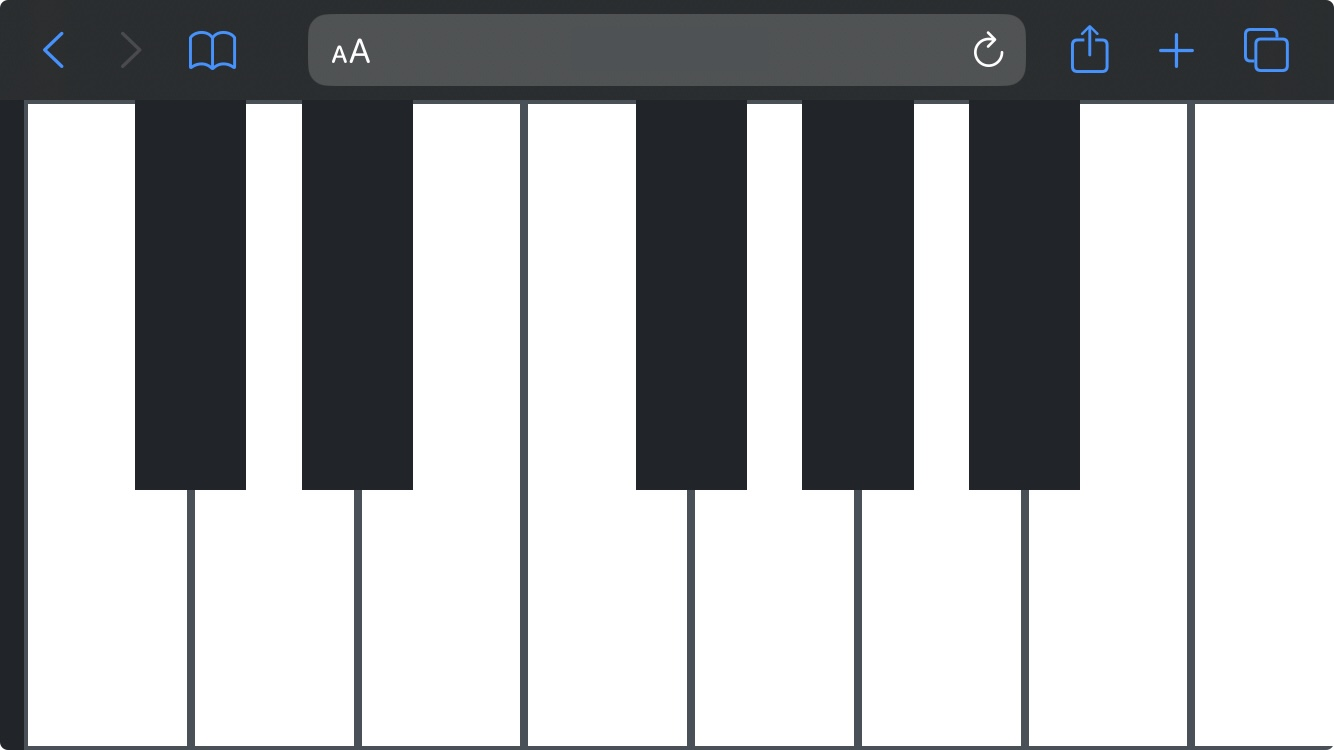
\includegraphics[width=0.65\textwidth]{images/Piano.jpeg}
    \caption{Captura de ecrã do dispositivo móvel, revelando a página web com uma oitava de um piano, ponte permite a participação do público na obra. \textsl{(A imagem foi editada de modo a esconder o IP disposto na barra de pesquisa.)}}
    \label{fig:Piano}
\end{figure}

Por outro lado, uma vez que o público tem sempre a oportunidade de utilizar a plataforma para criar objetos sonoros, é crucial que a intenção emocional e energética das assímptotas seja clara no discurso musical do intérprete, de modo a que não desperte a curiosidade mas sim a necessidade de conclusão de uma secção. Assim, é tão importante o florescer da curiosidade em cada membro do público como a sua ausência. 

Ao longo da obra, dividida em 5 exercícios, cada membro do público poderá pressionar uma tecla, produzindo resultados distintos dependendo da secção em que a peça se situa; estes comprimem desenhos monódicos, objetos sonoros singulares e manipulação tímbrica dos objetos criados pelo músico. No dispositivo móvel apenas constará um teclado com uma oitava de amplitude (Dó a Si), cuja oitava relativa é atribuída aleatoriamente sempre que o utilizador entra na página ou a recarrega.

As preparações, que serão processadas através do referido software \textsl{bitKlavier}, para se integrarem melhor enquanto extensão do piano, e não como instrumento secundário, são projetadas através de colunas de contacto que, tendo a caixa de som do piano como suporte, criam a desejada ilusão de que o som provém do piano. Mais ainda, uma vez que as colunas não estão muito visíveis, este sistema encaixa-se no conceito central da obra, relevando a curiosidade do público sobre a origem do som.

A ligação entre a curiosidade e as assímptotas nasce da dificuldade de previsão da carga energética do silêncio, a qualquer momento. Que som nasce do silêncio? Quanto tempo dura a tensão quando o silêncio rompe? Como é que o silêncio se insere após o caos? Estas retóricas são o combustível que alimenta o fluxo da obra, tanto na perspectiva de quem a observa como na de quem a interpreta.

Abraçando o espírito da obra, embora ela detenha um título, este nunca será divulgado. Opcionalmente, o intérprete também poderá usar uma capa e máscara para não ser reconhecido. Para garantir consistência, ao longo desta análise os termos \enquote{intérprete} e \enquote{músico} representam o performer que se encontra ao piano a interpretar a obra e o termo \enquote{público}, embora seja comumente atribuido aos indivíduos que apenas ouvem a obra, é aqui estendido, pois este também é participante na performance da obra.

\Subsection{Análise das secções}

Cada uma das secções é apresentada com um exercício performático criado propositadamente para a obra em questão. Devido à infinidade de possibilidades de tradução dos exercícios para vocabulário musical, para cada um são expostas duas interpretações escritas: uma dedicada à escrita em partitura, divulgada através do intérprete, e outra dedicada às preparações tocadas pelo público. No entanto, em todos os exercícios há uma componente de carácter improvisatório, que permite ao músico explorar novas interpretações sintáticas do seu conteúdo performático.

Para cada secção foi concebido um par de \textsl{patches}, mapas de preparações digitais que atentam eventos \textsl{MIDI} que as accionam. Estes \textsl{patches} conectam-se ao público, por meio da plataforma web, e ao intérprete, através de um controlador \textsl{MIDI}, preferencialmente com, pelo menos, 32 notas de amplitude e possibilidade de trocar entre oitavas. Cada \textsl{patch} do mesmo par tem uma estrutura idêntica, variando apenas em alguns parâmetros e, na análise de cada secção, é exposta uma imagem de um dos \textsl{patches}, juntamente com uma breve descrição do seu conteúdo e lista de tipos de preparações.

Para criar os referidos \textsl{patches}, é necessário criar os grafos de preparações manualmente, inserindo os parâmetros em cada preparação, como é possível observar na Figura \ref{fig:bitsync}. Na maioria das preparações, estes parâmetros podem ser definidos através da \textsl{UI}\footnote{\textsl{User Interface} (Interface do utilizador)} ou por edição numérica. No caso de preparações como a Resonance, onde não é possível manipular numericamente os parâmetros, há a possibilidade de importar os parâmetros através de um ficheiro externo.

\begin{figure}[h]
    \centering
    \captionsetup{width=0.8\textwidth}
    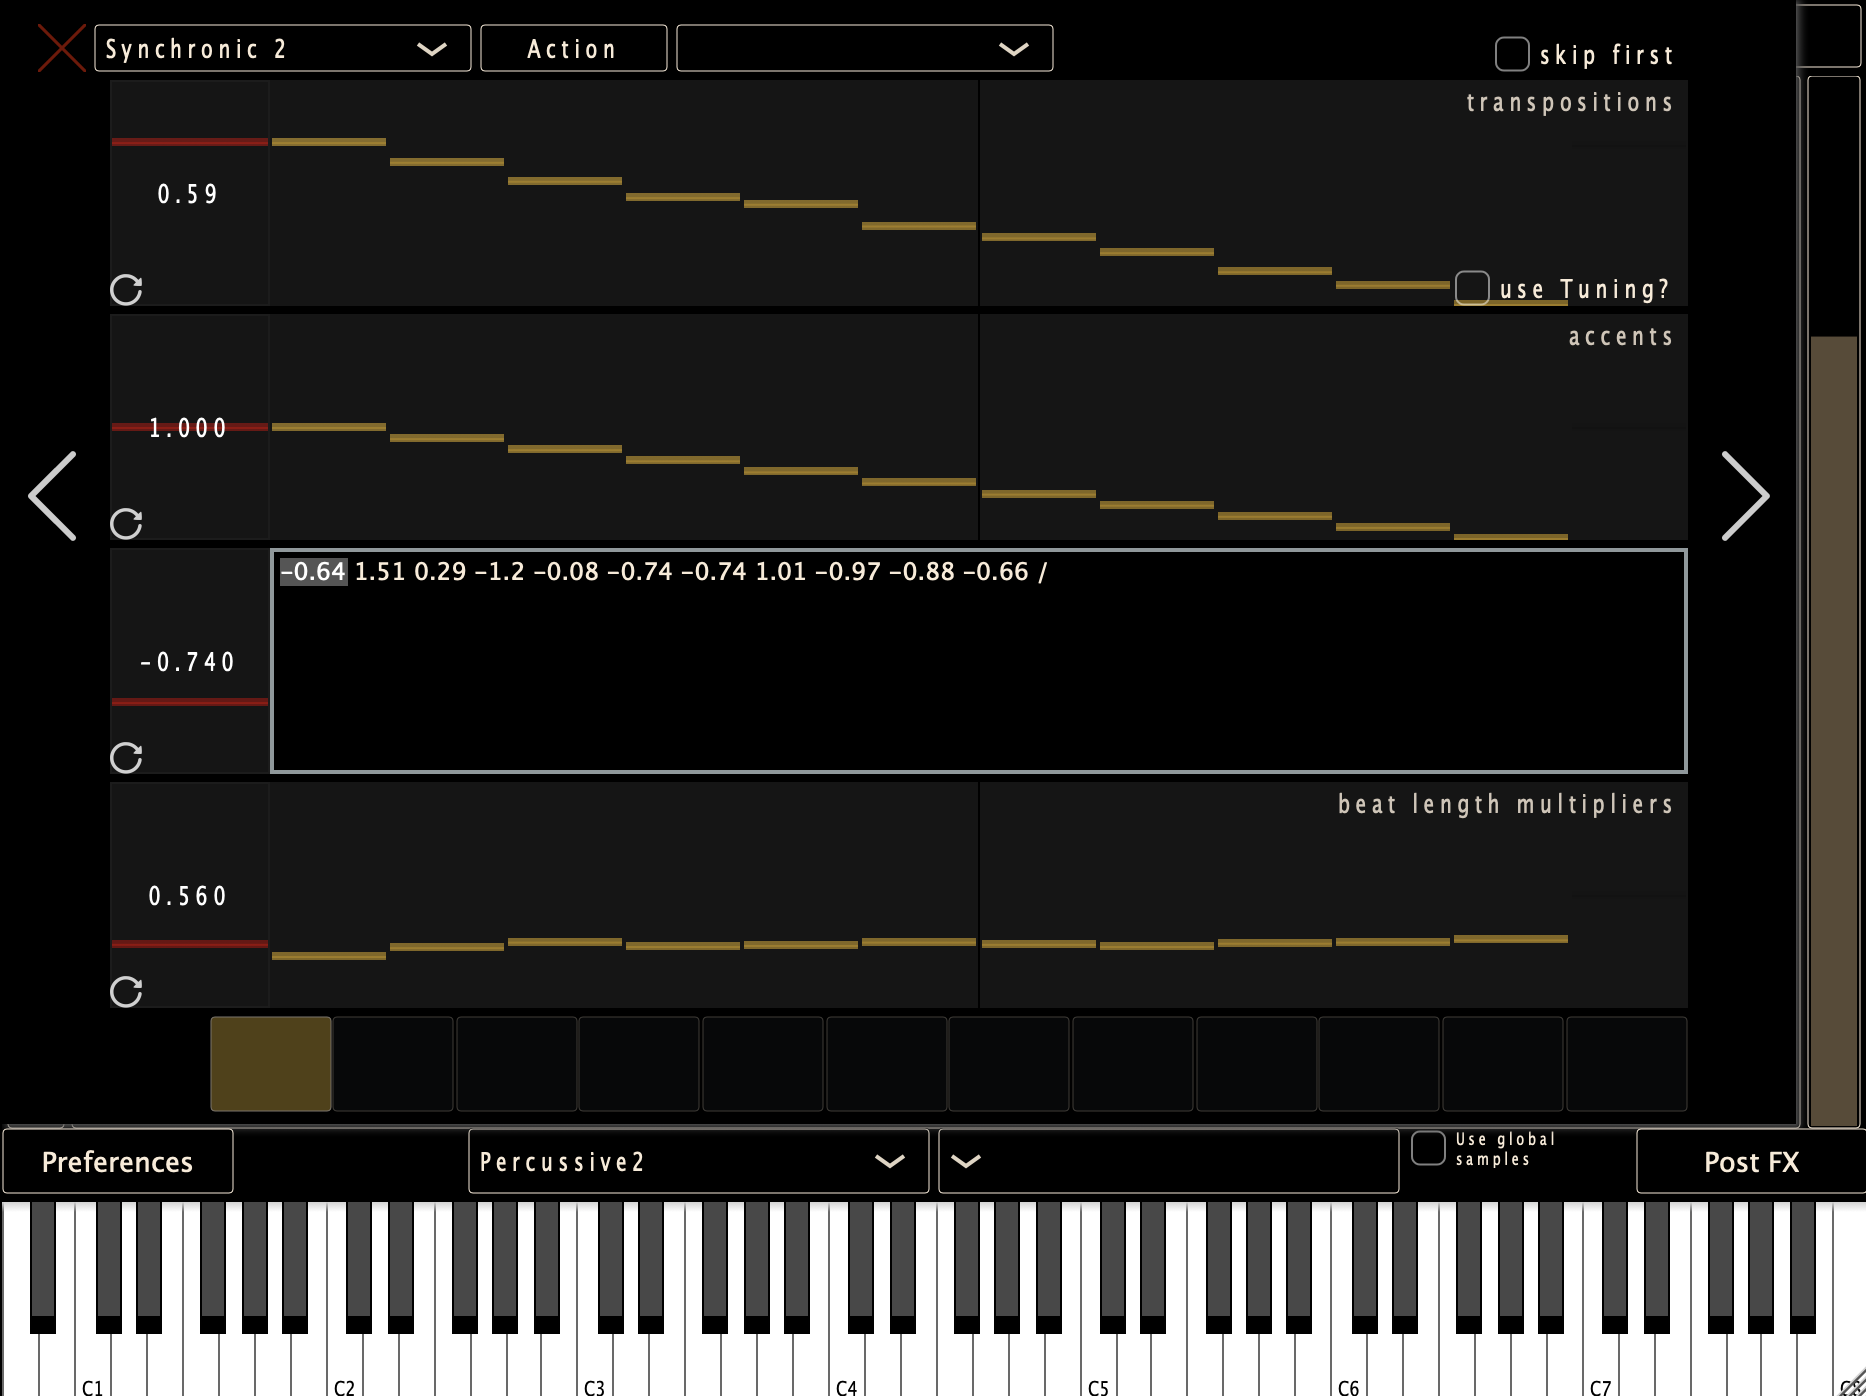
\includegraphics[width=0.7\textwidth]{images/bitsync.png}
    \caption{Menu de edição de parâmetros de uma preparação Synchronic. Utilizando a \textsl{UI}, os vários \textsl{steps} podem ser alterados, por arraste com o rato, ou editados numericamente, quando o utilizador faz \textsl{double click} por cima do campo desejado.}
    \label{fig:bitsync}
\end{figure}

Cada Gallery, Piano ou preparação é gravada como ficheiro \textsl{XML}\footnote{\textsl{Extensive Markup Language}}, permitindo assim a manipulação de parâmetros, ou outras opções de funcionamento, através da alteração do próprio ficheiro, utilizando qualquer software de edição de texto. Isto permite extender a amplitude de possíveis parâmetros, como é o caso das preparações Resonance, onde, no presente trabalho, foi construído um código simples para gerar instâncias desta preparação com parâmetros pseudo-aleatórios, como se pode ver no Anexo I. Após gerar o ficheiro \textsl{XML}, é possível importar esta configuração a partir do menu de edição dos parâmetros.

Outro elemento chave na criação dos \textsl{patches} é a atribuição de instrumentos digitais a cada preparação. Embora o software já ofereça um conjunto próprio, para este projeto foram sintetizados novos instrumentos, de modo a providenciar não só uma coleção cuja complexidade é desconhecida para o intérprete, como também alcançar características tímbricas únicas e detalhadas para cada secção da obra. O código para geração dos instrumentos encontra-se disponível no Anexo II.

Relativamente à musicografia, todas as secções apresentam o exercício escrito e um sistema com um pentagrama para as preparações e um ou dois pentagramas para o piano, sendo que as preparações deverão ser tocadas através do referido controlador \textsl{MIDI} e não representam o resultado sonoro, apenas a nota a ser premida. Também estão registadas algumas indicações de interpretação e improvisação, porém de uma forma não muito objetiva para permitir um evolução imprevisível do discurso musical e para não influenciar o intérprete na sua expressão artística dos exercícios. Pela mesma razão, e recuperando o conceito da obra, nem todas as indicações se encontram disponíveis na partitura, estimulando o sentimento de curiosidade por parte do músico para procurar mais informação sobre a peça.

\Subsubsection{0 - O Início?}
\begin{performex}
    Um performer, em completa solidão, entra numa sala vazia, com um objeto imaginário na mão. Após colocar o objeto no chão, senta-se e contempla-o na sua quietude. O exercício termina quando o performer sentir que o objeto escapou à sua imaginação, desmaterializando-se.
\end{performex}

A secção número 0 não se encontra em partitura. Representa, no entanto, o exercício performático literal que o intérprete deverá praticar antes da performance da obra, enquanto preparação artística. Noutra perspectiva, simboliza a presença do silêncio na música: o performer é a fonte sonora e da sua imaginação provém o objeto sonoro que ele produz, com uma carga emocional e energética que apenas o performer conhece, porém ninguém se encontra lá para observar.

Aquando do término do exercício, o músico coloca um envelope fechado no chão, cujo conteúdo é referido na secção 6, e senta-se ao piano, esperando a entrada do público na sala.

\Subsubsection{I - Imitação Cega}
\begin{performex}
    Dois performers encontram-se de costas um para o outro. À vez, um deles terá de fazer um movimento juntamente com um som que descreve o próprio gesto, e o outro terá de o copiar. Este exercício pode ser expandido de duas formas distintas. Numa, cria-se uma linha de performers que cada um tem de imitar o gesto e som feito pela pessoa que está atrás; noutra variante, um performer encontra-se de olhos vendados no centro de um círculo criado por vários performers, onde cada um, não necessariamente à vez, cria o seu movimento e som, que irá repetir ao longo do exercício, enquanto o performer do meio vai copiando os diversos estímulos que recebe.
\end{performex}

A primeira instância deste exercício ocorre quando o intérprete toma o papel do performer que se encontra no centro do círculo a tentar copiar, musicalmente através da improvisação, os gestos sonoros realizados pelas preparações, por meio do público. Após algumas repetições, o público deixa de ter controlo direto sobre os objetos sonoros e o exercício toma a variante inicial com apenas dois performers de costas um para o outro, i.e., piano versus preparações. Aqui, já seguindo a partitura escrita, as preparações tocam uma monodia quebrada que é posteriormente imitada pelo piano. De seguida o piano desenvolve o discurso musical e as preparações iniciam a imitação, interrompendo o gesto, culminando num jogo de espelhos entre ambos os instrumentos.

Tratando-se de imitação, a repetição enquanto espelho tem um papel muito forte nesta primeira secção. Uma vez que se trata de uma imitação conduzida apenas pela audição, dentro dos domínios musicais todos eles são alvo desta imitação, sendo ainda assim encorajada a tradução das características performáticas de um dos domínios para outro distinto durante a secção improvisatória. Um exemplo seria escutar um gesto musical cujas notas crescem gradualmente em frequência e a respectiva imitação ser uma única frequência crescer gradualmente em aplitude.

Por outro lado, a quietude inerente à espera e escuta, anterior à fase de imitação, também é crucial para o desenvolvimento do exercício, pois o performer pode escolher aprofundar a quietude antes de repetir, ou até encurtar a espera, interrompendo o outro performer. É através desta quietude que é explorada a referência às diversas assímptotas: é por meio do silêncio de um performer que o outro sabe que o objeto performático terminou, que o estado de quietude se iniciou e que a repetição pode ser explorada. Mais ainda, mesmo existindo silêncio, a qualidade performática do elemento artístico pode sugerir uma carga energética forte ou fraca o suficiente para a quietude do performer que a escuta se alongar ou encurtar, respectivamente.

O \textsl{patch} (Figura \ref{fig:bit1}) concebido para esta secção é o mais complexo, pois necessita carecer previsibilidade para estimular a criatividade de improvisação. Cada uma das notas da oitava poderá ter uma das seguintes configurações:
\begin{itemize}
    \item Duas preparações Synchronic de parâmetros aleatórios, onde um tem um instrumento de carácter mais melódico e outro mais percussivo.
    \item Uma preparação Direct com um instrumento melódico, ligado a uma preparação Blendronic de parâmetros aleatórios.
    \item Uma preparação Nostalgic com um instrumento melódico, ligado a uma preparação Blendronic de parâmetros aleatórios.
\end{itemize}
As preparações accionadas pelo controlador \textsl{MIDI} passam por uma preparação Direct, que está ligada a todas as preparações Blendronic presentes no \textsl{patch}.

\begin{figure}[h]
    \centering
    \captionsetup{width=0.8\textwidth}
    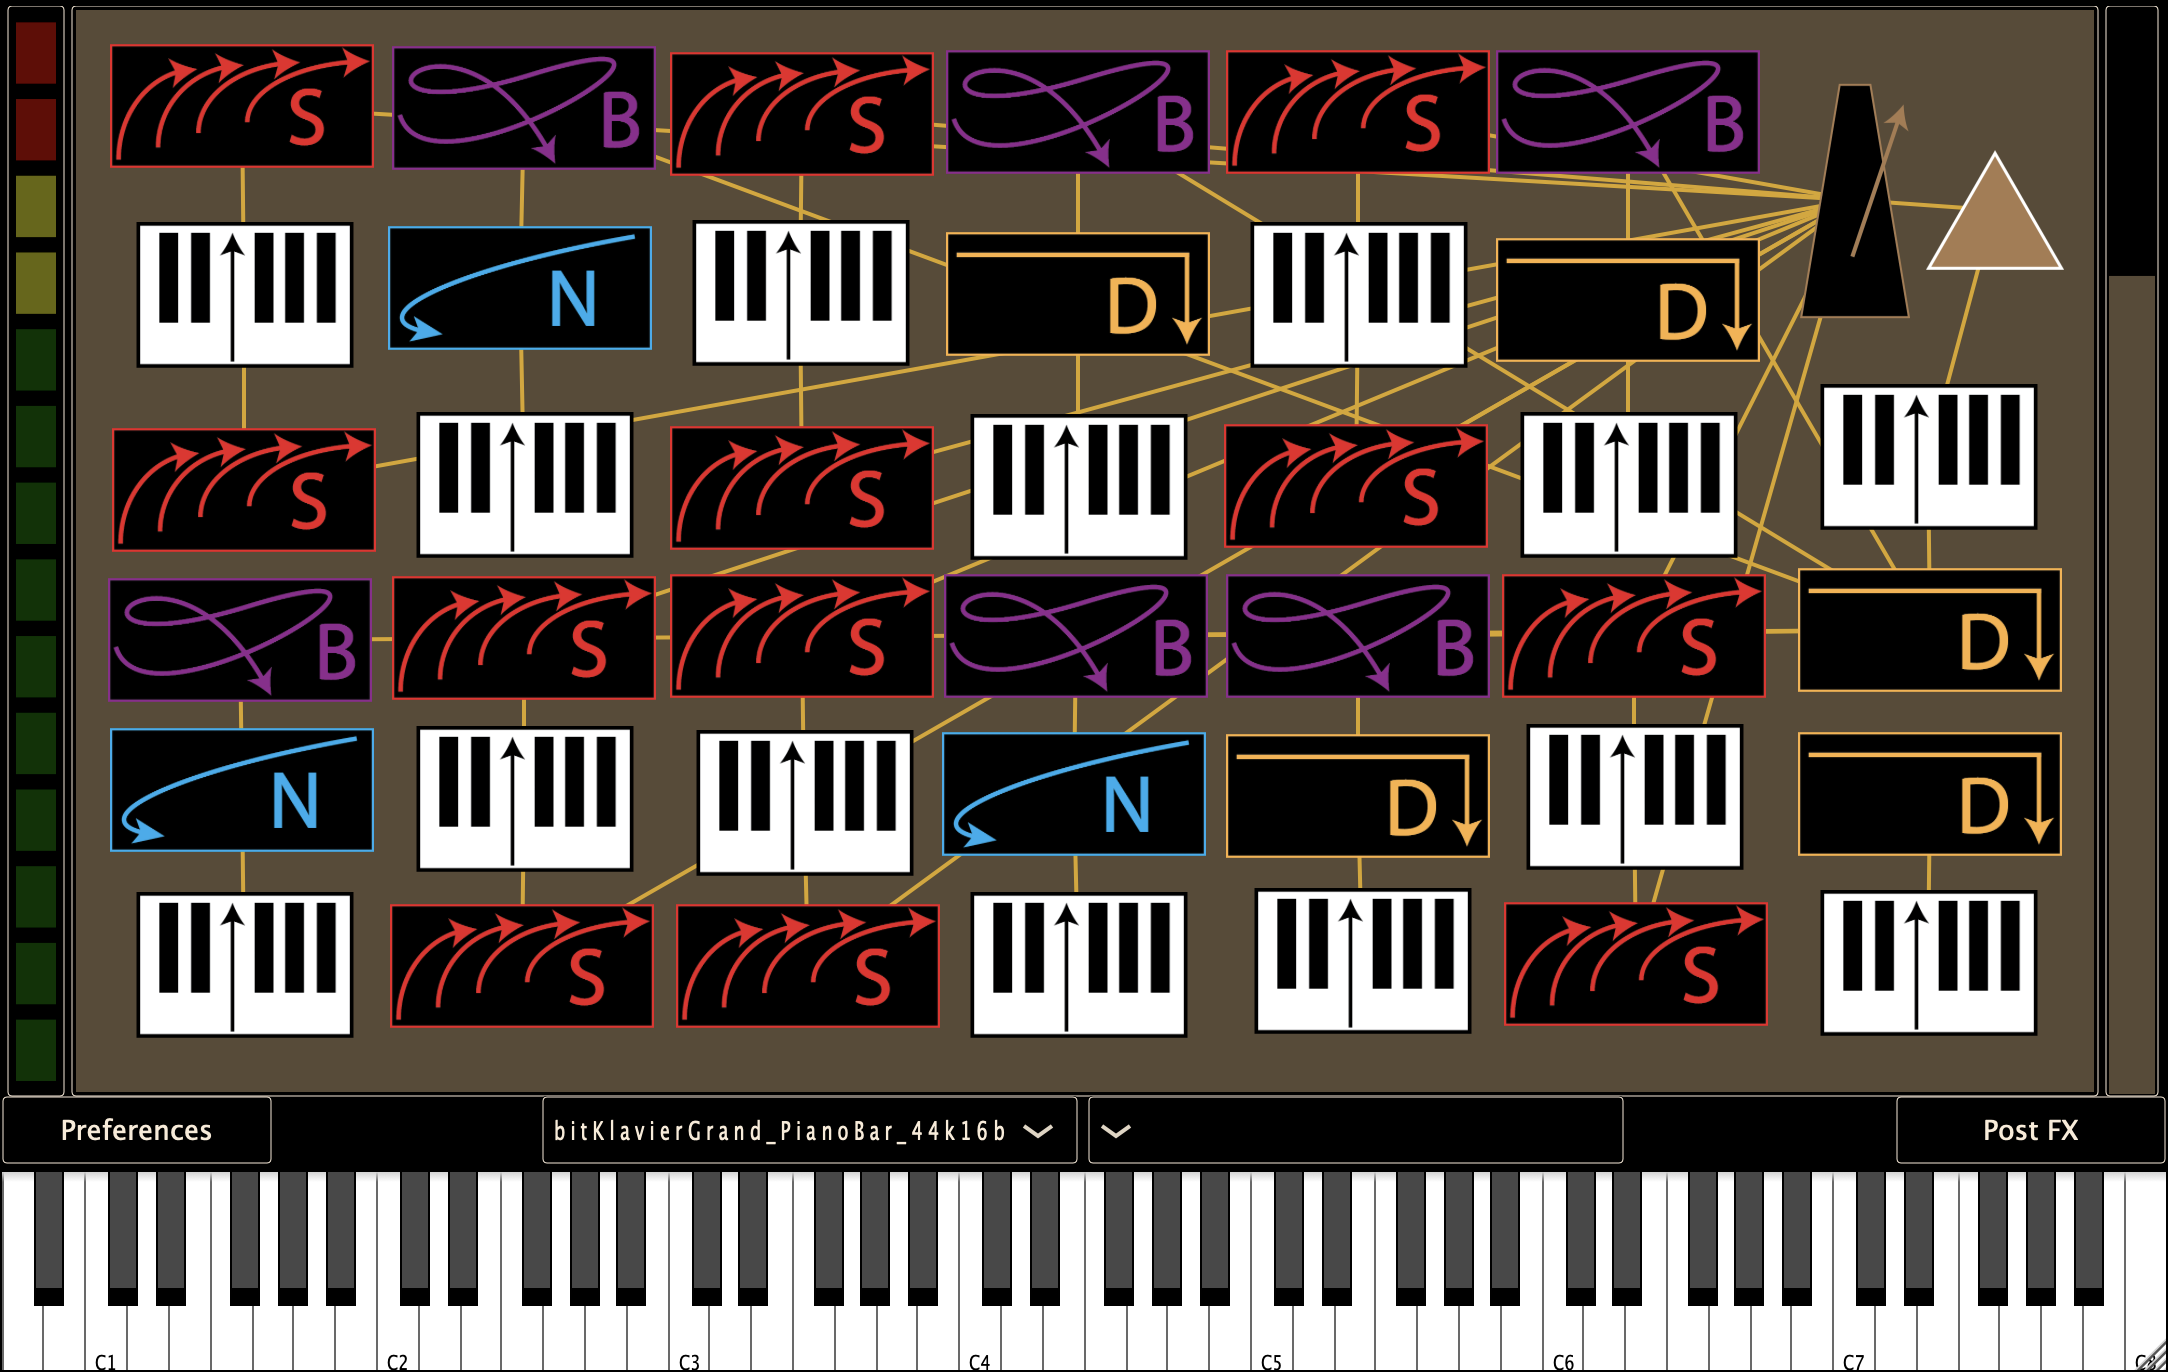
\includegraphics[width=0.7\textwidth]{images/bit1.png}
    \caption{\textsl{Patch} das preparações da primeira secção da obra. Cada nota tem uma das 3 configurações distintas, todas com parâmetros aleatórios, garantido um sistema de preparações complexo o suficiente para inibir previsibilidade.}
    \label{fig:bit1}
\end{figure}

Devido à natureza das preparações Blendronic, o som resultante da fração inicial de improvisação é reflectido pelas preparações, numa textura musical muito semelhante ao discurso exposto na partitura (Figura \ref{fig:obra1}), simulando a repetição referida no exercício performático.

\begin{figure}[h]
    \centering
    \captionsetup{width=0.8\textwidth}
    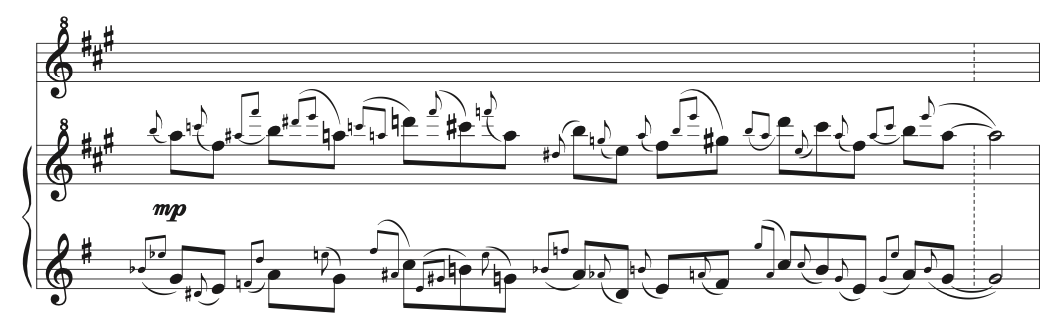
\includegraphics[width=0.7\textwidth]{images/obra1.png}
    \caption{As duas monodias, em homorritmia e separadas por um intervalo constante (quietude), desenham o mesmo contorno melódico (repetição em espelho), quebrado pela presença contrastante das figuras rápidas (inconsistência), que também procuram copiar a textura das preparações Blendronic (repetição em cópia).}
    \label{fig:obra1}
\end{figure}

Na segunda fração dedicada ao texto improvisado, as figuras rápidas não estão especificadas na partitura, para encorajar uma cópia mais fiel ao discurso das preparações. Gradualmente, e com o declínio natural dos Blendronic's ativos, é alcançado o silêncio através de uma assímptota, tomada arbitrariamente pelo músico no decorrer da performance, de acordo com o que achar mais adequado a nível energético e emocional.

\Subsubsection{II - Montagem}
\begin{performex}
    Um grupo de performers encontra-se em círculo largo, com um performer no centro de olhos vendados. Após 15 pulsações internas, um intérprete desloca-se de forma livre até ao performer no centro, congelando no momento em que toca nele. Sequencialmente, os restantes performers fazem o mesmo, podendo deslocar-se para qualquer uma das pessoas congeladas no centro. Ao fim de todos estarem no centro, o exercício pode terminar ou então movimentar-se como um único corpo pelo espaço.
\end{performex}

Neste exercício a parte escrita é a primeira a ser executada. Aqui, os 3 vocábulos da arte performática estão expostos: quietude no início, no grupo que está no centro e nos performers que esperam a sua vez, repetição no ato de quebrar a quietude do círculo para atingir a quietude do centro e inconsistência no movimento de cada performer. O domínio da frequência representa o estado de cada performer, principalmente na harmonia vertical representada pelo aglomerado que está no centro. 

A quietude inicial parte do silêncio obtido pela assímptota do espaço, quebrada pela aproximação do som por meio de gestos sugestivos do intérprete, revelando que a quietude do performer se mostra pela frequência, uma vez que cada desenho monódico se inicia numa nota distinta. Estes representam o movimento até ao centro que, pela sua inconsistência natural, são explorados por todos os domínios sonoros, atingindo novamente a quietude. Esta, demonstrada na harmonia situada no final de cada gesto, também inere uma certa inconsistência devido ao crescimento do aglomerado de performers como um só corpo, que é manifestada através de alterações tímbricas do conjunto harmónico, como é possível ver na Figura \ref{fig:obra2}.

\begin{figure}[h]
    \centering
    \captionsetup{width=0.8\textwidth}
    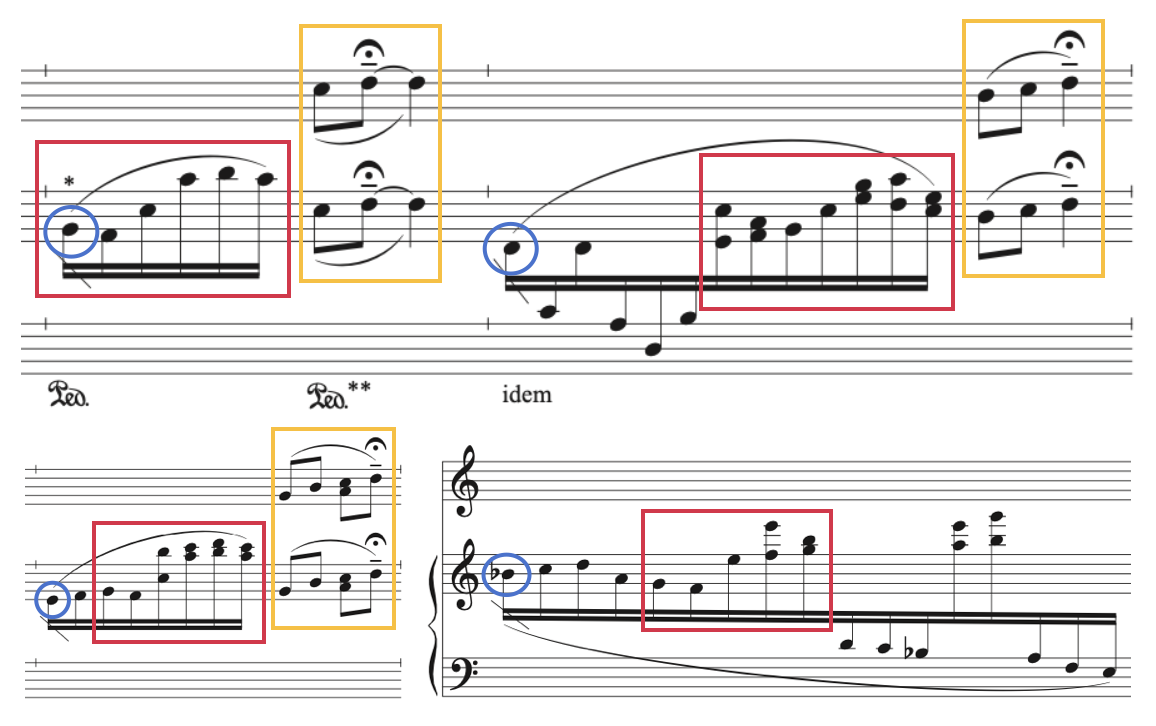
\includegraphics[width=0.7\textwidth]{images/obra2.png}
    \caption{Excertos da secção 2, onde é possível observar as diferentes notas iniciais (círculo azul), a repetição do exercício em sobreposição com a inconsistência dos movimentos (rectângulo vermelho), e a quietude presente na harmonia do aglomerado (rectângulo amarelo).}
    \label{fig:obra2}
\end{figure}

A parte improvisatória desta secção situa-se na última parte do exercício, ou seja, o movimento do aglomerado como um todo e, posteriormente, o repouso. Enquanto que o intérprete toca de um modo inconsistente a harmonia, quebrando entre o piano e as preparações, o público toma o controlo sobre a qualidade tímbrica do som, descrevendo também os seus movimentos, adicionando objetos às preparações e alterando o espetro do resultado harmónico.

\begin{figure}[h]
    \centering
    \captionsetup{width=0.8\textwidth}
    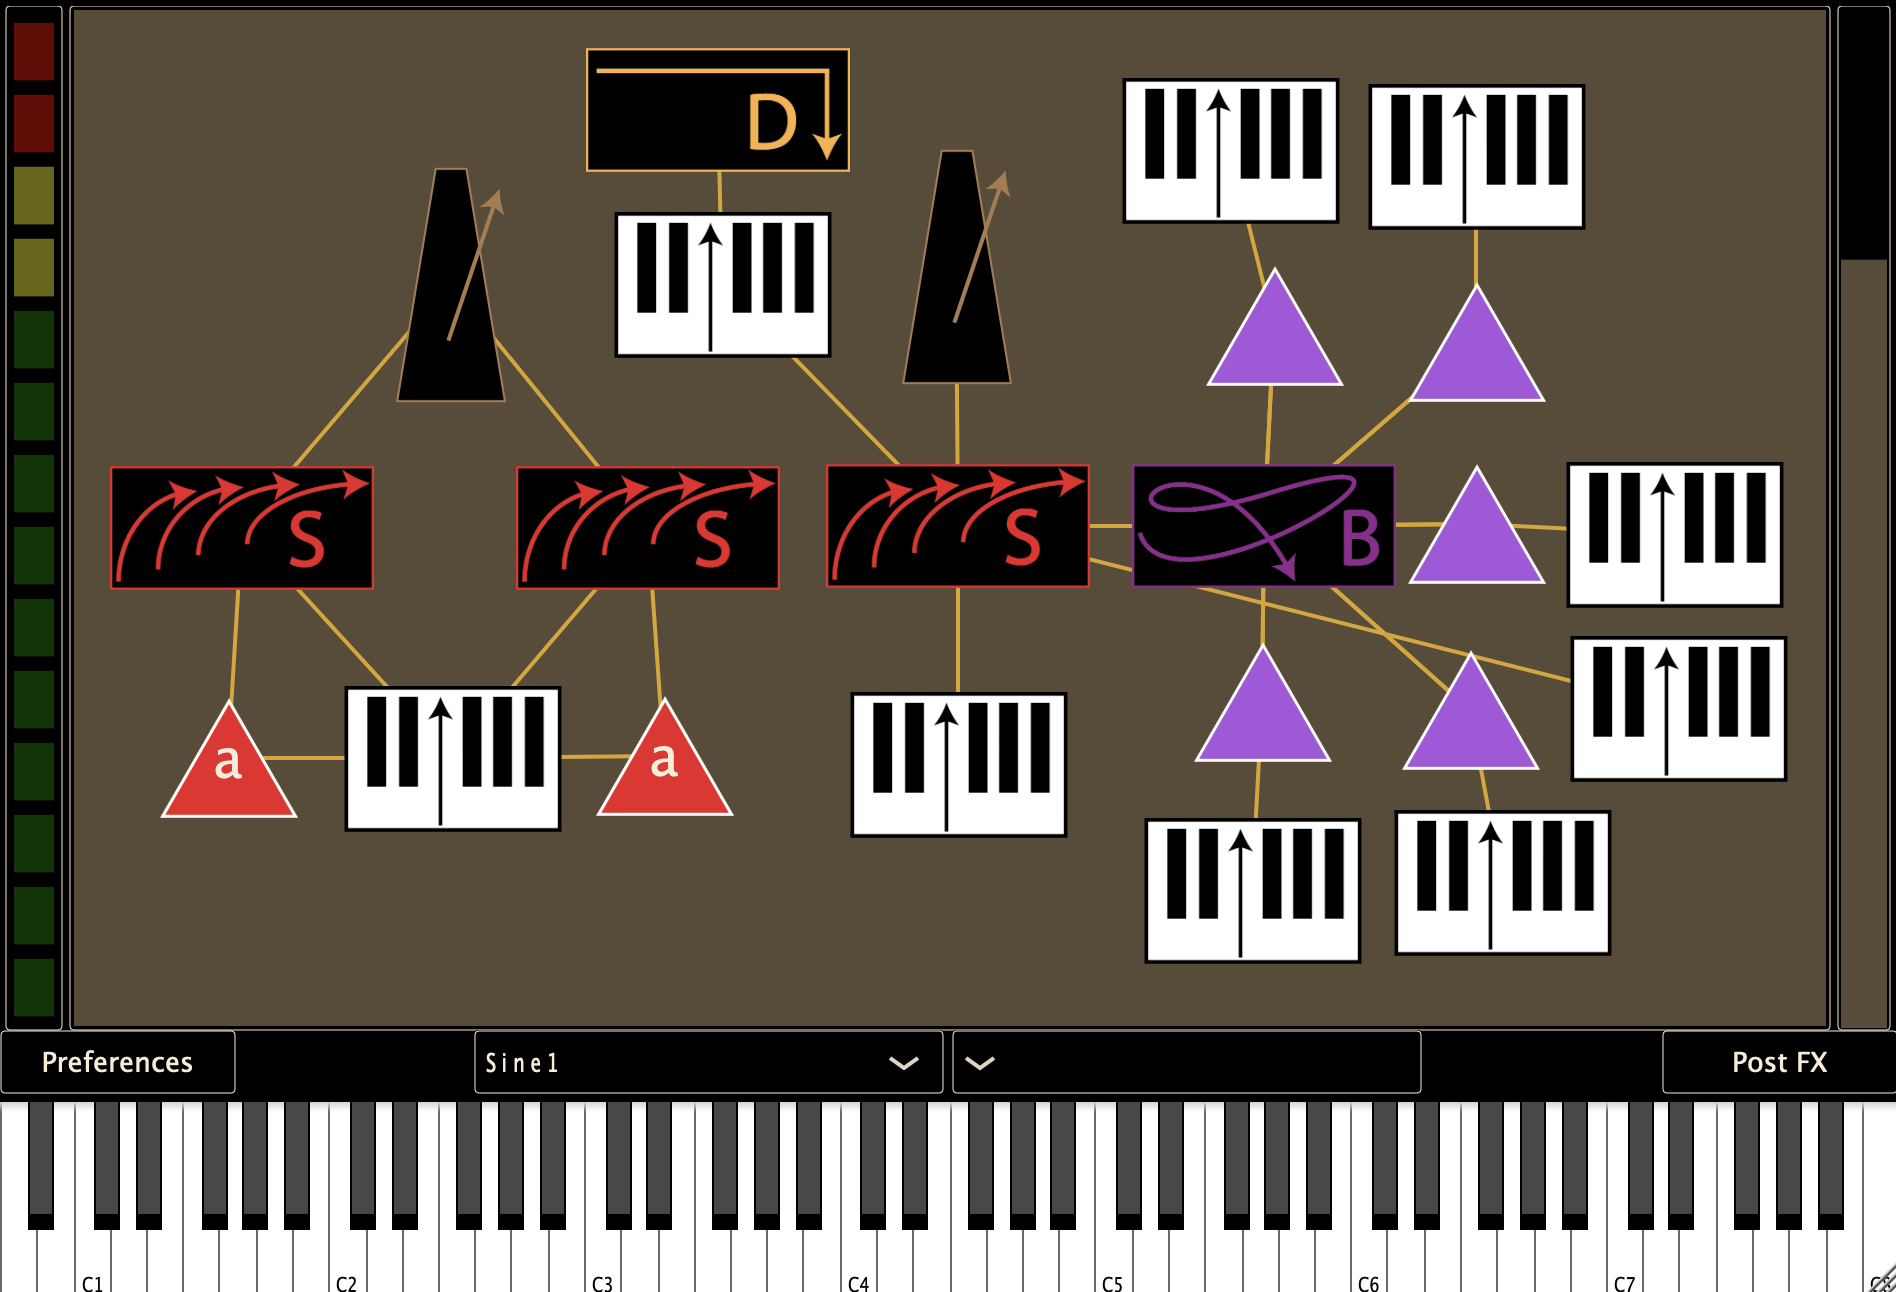
\includegraphics[width=0.7\textwidth]{images/bit2.png}
    \caption{\textsl{Patch} da secção 2. É possível reparar que o sistema é composto por dois grafos desconexos: o da esquerda representa o performer no meio do círculo, estando mapeado apenas para a nota Ré, e o da direita modela o registo tímbrico da harmonia do aglomerado e as respectivas alterações, utilizando Modifications controladas pelo público.}
    \label{fig:bit2}
\end{figure}

Este sistema é conseguido através de Keymaps ligados às preparações Synchronic, com o objetivo de adicionar notas ao aglomerado harmónico, e com Modifications que alteram os parâmetros das preparações Blendronic (Figura \ref{fig:bit2}). Gradualmente, o músico exclui algumas notas do aglomerado, terminando a secção através da aproximação do silêncio pela assímptota do timbre.

\Subsubsection{III - Elos}
\begin{performex}
    Um grupo de número par de performers posiciona-se em círculo, todos virados para dentro do mesmo, com os olhos fechados. Após 15 pulsações internas, quebram a sua quietude, movendo o corpo lenta e livremente. A qualquer momento um performer pode abrir e fechar os olhos, porém se cruzar olhares com outro performer, ambos congelam na posição em que se encontram, mantendo o contacto visual. Quando todos estiverem bloqueados, aprofundam a quietude, fechando posteriormente os olhos e colocando-se numa posição de repouso.
\end{performex}

Neste exercício, o caos emerge da quietude. Os movimentos independentes são uma expressão totalmente imprevisível da inconsistência, detendo alguns elementos repetitivos como o abrir e fechar de olhos. Aos poucos, a quietude surge quando elos visuais são criados, congelando a tensão característica do exercício performático.

Na obra, esta secção não tem parte escrita, apenas alguns guias visuais para o perfil textural do discurso musical de carácter improvisatório. O objetivo do músico é realizar sons o mais inconsistentes possível a nível dos domínios primários da frequência e amplitude e no domínio psicoacústico da métrica, mantendo a quietude de timbre, espaço e pulsação. De um modo livre, o \enquote{abrir-fechar de olhos} é traduzido num gesto de repetição reversa causada pelas preparações, dentro do domínio do timbre.

O público também realiza este passo, sendo que sempre que o registo tímbrico das preparações do público for idêntico ao das preparações do músico, o estado da catexia ativa da diferença move-se ao longo do seu eixo, em direção à repetição, num dos domínios sonoros que se encontram no estado de inconsistência. Assim que esta catexia se encontrar predominantemente na repetição, as preparações deixam de soar e o estado energético da catexia ativa do desenvolvimento desloca-se ao longo do seu eixo, em direção à subtração, até ser atingido o silêncio pela assímptota do tempo.

Uma vez que tanto o público como o músico partilham funções no que toca às preparações, e como tal se limita apenas ao \enquote{abrir-fechar de olhos}, este \textsl{patch} (Figura \ref{fig:bit3}) é o mais simples da obra, sendo composto por apenas uma preparação Synchronic (ligada a um Metronome) e uma preparação Nostalgic. O produto sonoro criado pelas preparações utiliza ambas as assímptotas do tempo e do espaço, transladando-se em linha reta pelos eixos \enquote{futuro-presente-passado} e \enquote{longe-perto-longe}, concebido pela presença do Nostalgic em diálogo com o Synchronic. Existe aqui um paralelismo entre o silêncio e a visão de cada performer, pois, embora todos os performers tenham olhos (energia performática), as suas pálpebras (assímptotas) impedem a concretização da imagem (objeto sonoro); o ato de abrir os olhos simboliza a passagem do silêncio para o som através das assímptotas.

\begin{figure}[h]
    \centering
    \captionsetup{width=0.8\textwidth}
    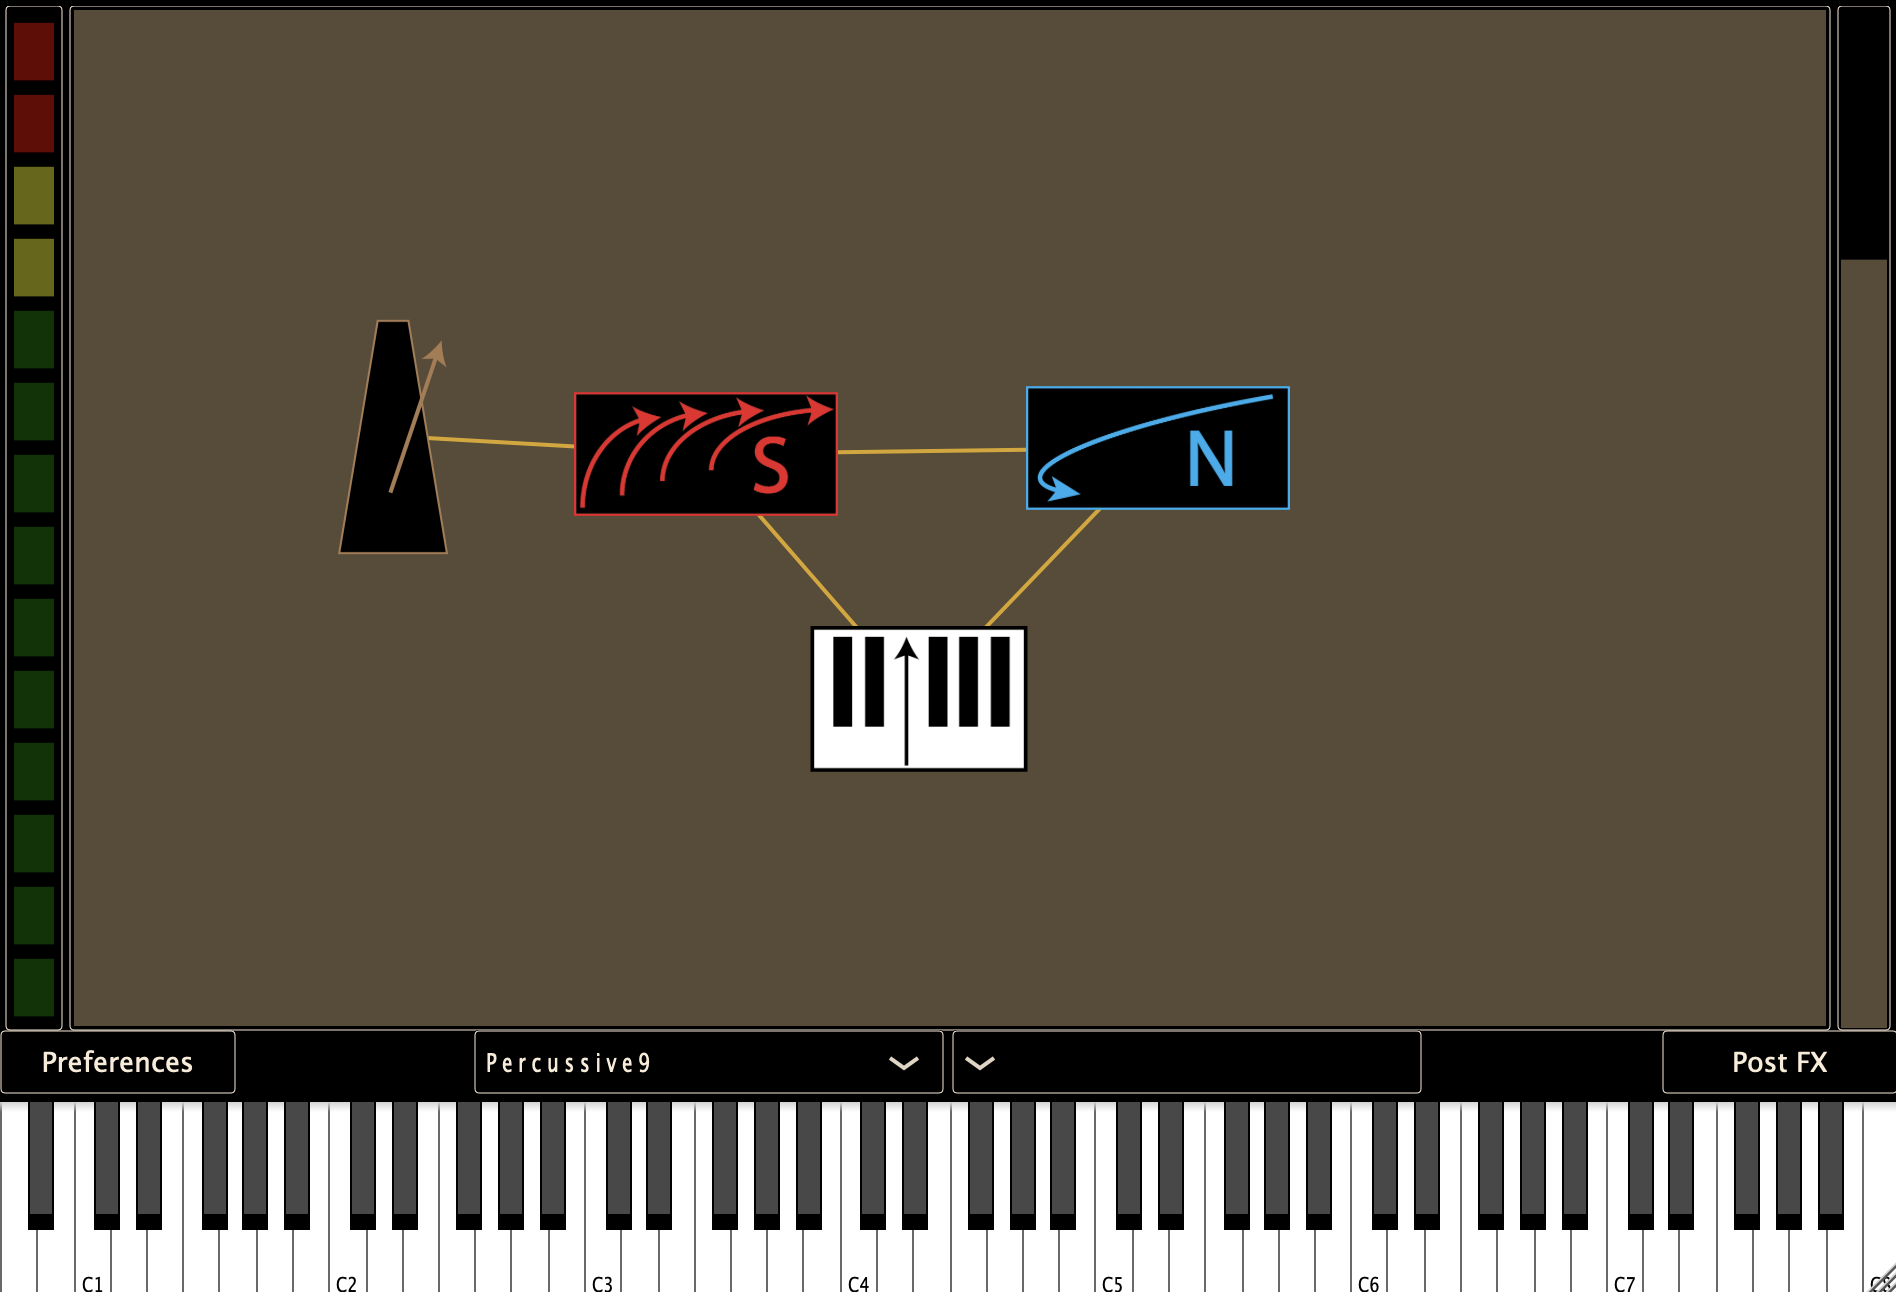
\includegraphics[width=0.7\textwidth]{images/bit3.png}
    \caption{\textsl{Patch} da secção 3, composto apenas por um Synchronic, um Metronome e um Nostalgic. Neste sistema é explorada uma funcionalidade do software que consiste na ligação entre o Synchronic e Nostalgic, permitindo sincronizar o movimento inverso de uma preparação com as pulsações da outra.}
    \label{fig:bit3}
\end{figure}

\Subsubsection{IV - Qual é o oposto de um \enquote{piano}?}
\begin{performex}
    Dois performers encontram-se de frente um para o outro. Saíndo da quietude em que se encontram, um dos performers realiza gestos, movimentos e sons inconsistentes, mantendo-se sempre virado para o outro performer. Este, terá de fazer de "anti-espelho" em tempo real, isto é, um conjunto de elementos performáticos que expressam a maior antítese possível, face aos movimentos do primeiro performer. Este exercício pode ser amplificado tendo um grupo de performers a realizar a antítese de um único performer no centro de um círculo.
\end{performex}

Havendo duas versões deste exercício performático, uma delas será explorada na parte escrita da secção e a outra na parte improvisada. Porém, em ambos os casos, a sintaxe performática consiste numa inconsistência repetidamente consistente, uma vez que um performer está a tentar espelhar o outro da pior maneira possível. A nível musical, tal é expresso por meio de repetição e inconsistência em diferentes domínios sonoros; no caso da parte escrita, a frequência, amplitude e tempo são o alvo da inconsistência enquanto que espaço e timbre encontram-se repetidamente em discordância (Figura \ref{fig:obra4}).

\begin{figure}[h]
    \centering
    \captionsetup{width=0.8\textwidth}
    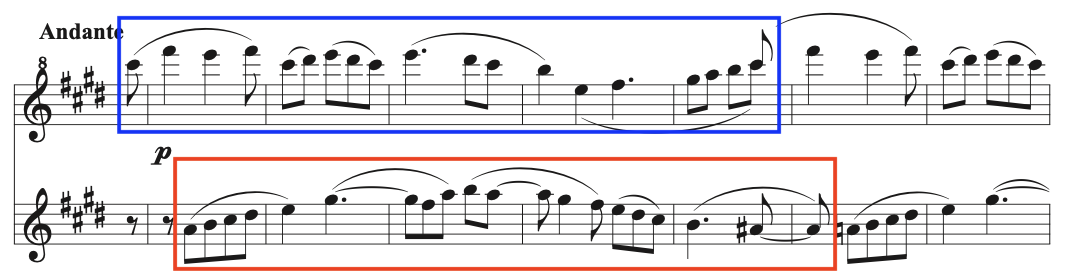
\includegraphics[width=0.7\textwidth]{images/obra4.png}
    \caption{Início da secção 4, onde ambas as linhas monódicas apresentam registos de frequência, dinâmica de fraseados e motivos rítmicos de um modo inconsistente. A nível de espaço e timbre, cada linha situa-se constantemente em discordância, uma vez que a linha inferior é sempre tocada no piano, ao contrário da linha superior. Mais ainda, o ato de cópia em tempo real é verificada no ligeiro desalinhamento das duas melodias.}
    \label{fig:obra4}
\end{figure}

Ao longo de todo o exercício, o público acciona as preparações de ressonância. Aqui, a antítese inerente à performance disponibiliza-se através de vibrações simpáticas artificiais, que constroem um espectro tímbrico e posteriores transformações do mesmo que constrasta com a textura do material produzido pelo músico.
O \textsl{patch} (Figura \ref{fig:bit4}) relativo a esta secção é composto por 5 preparações Resonance, cada uma ligada a 2 preparações Blendronic; enquanto que o Keymap que atenta os eventos \textsl{MIDI} do público está ligado às Resonances para disponibilizar as vibrações simpáticas, estas só ressoam quando as notas pressionadas pelo controlador \textsl{MIDI} do intérprete pertencem ao campo de ressonância de uma das preparações. Isto permite uma manipulação tímbrica da linha melódica destinada às preparações.

\begin{figure}[h]
    \centering
    \captionsetup{width=0.8\textwidth}
    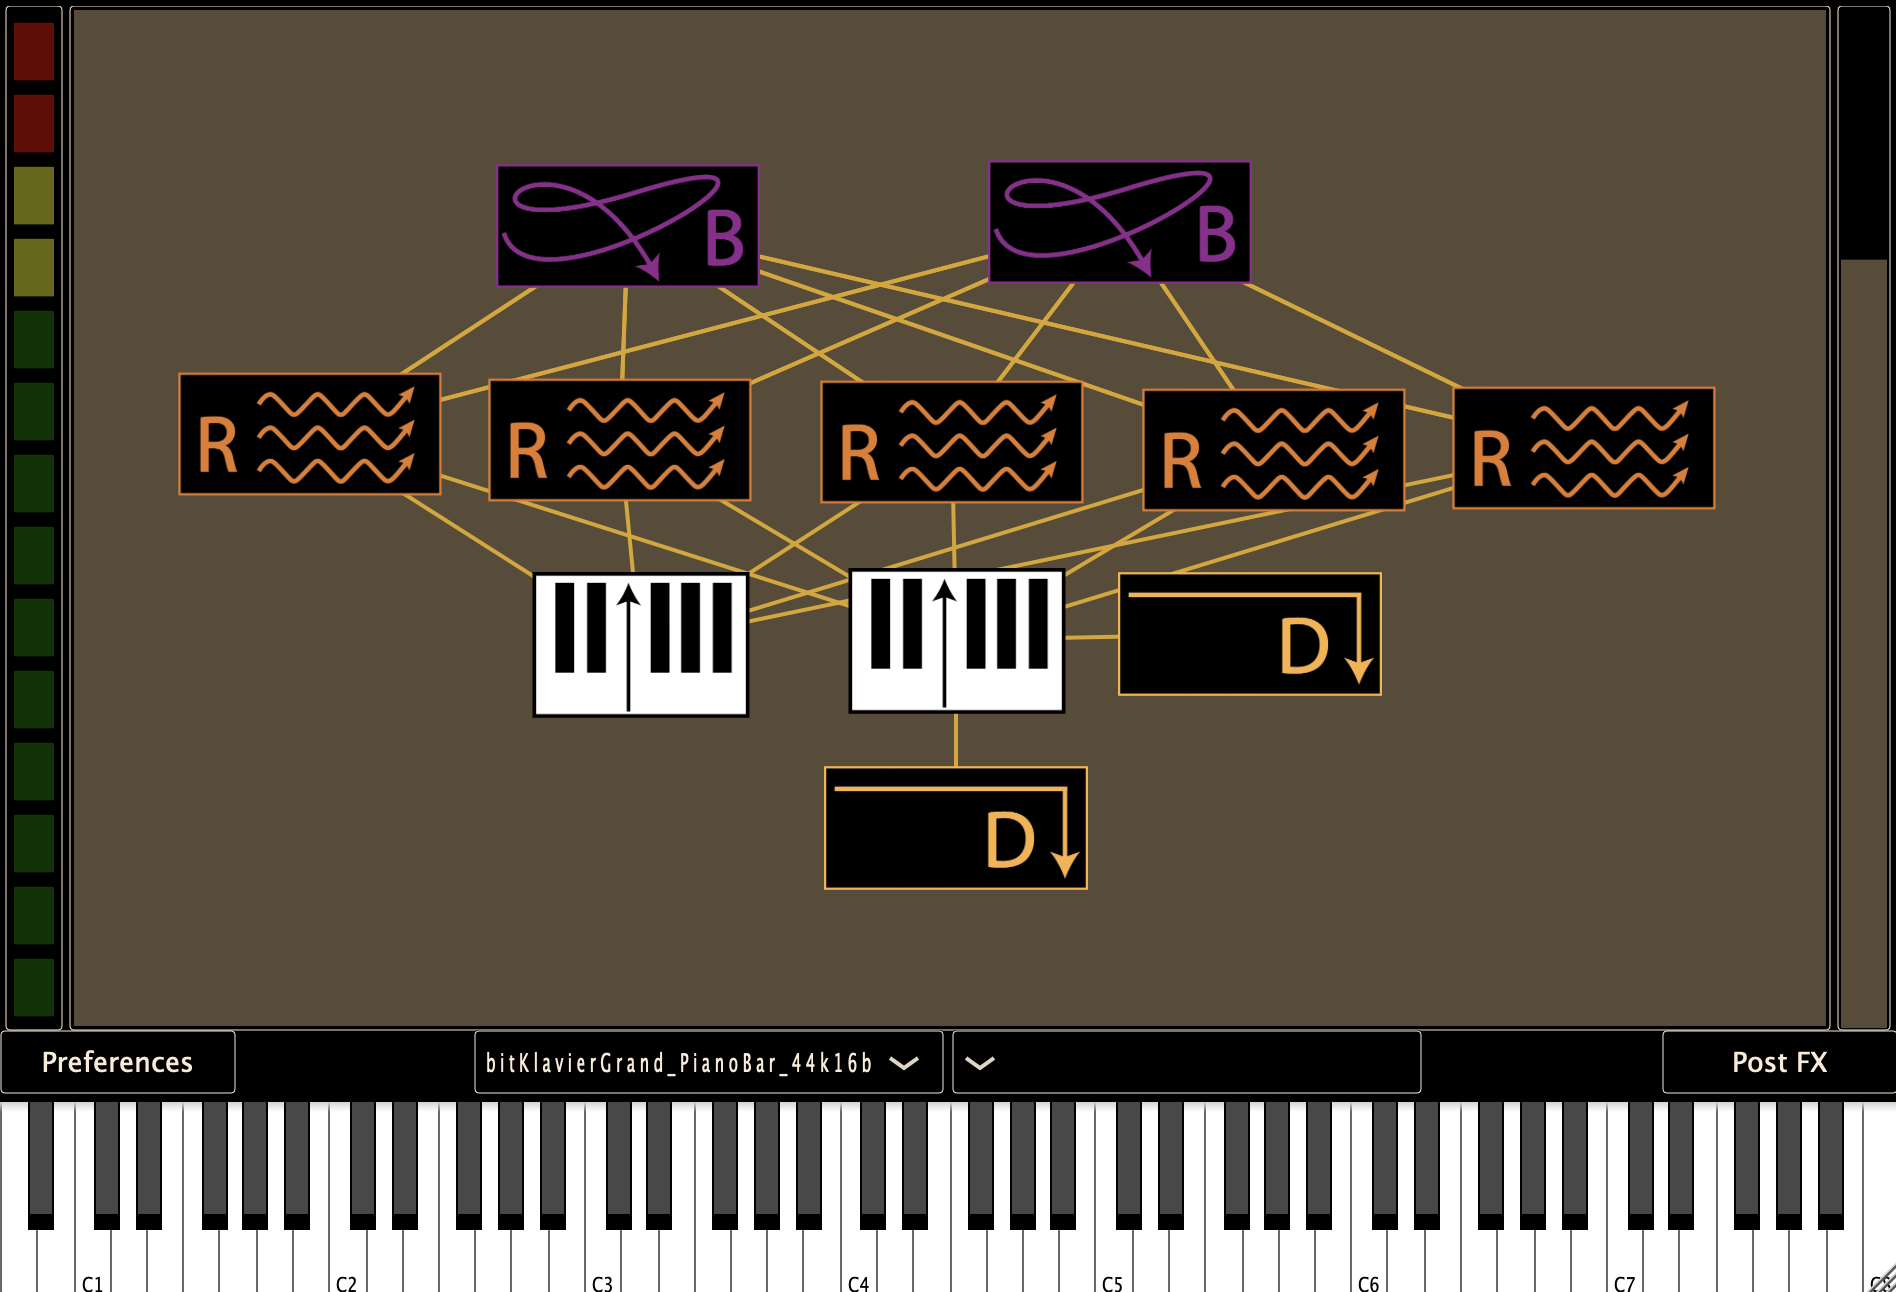
\includegraphics[width=0.7\textwidth]{images/bit4.png}
    \caption{\textsl{Patch} da secção 4, onde 2 Keymaps ligados a 5 Resonances têm a função de Add (Keymap do público), para adicionar notas ao campo de ressonância, e Ring (Keymap do músico), para iniciar a vibração das notas que fazem parte desse campo. Um par de preparações Blendronic enriquecem a complexidade tímbrica do resultado sonoro, contribuindo assim para a inconsistência característica do exercício.}
    \label{fig:bit4}
\end{figure}

Ao longo da improvisação, o músico, que apenas tocará piano, terá de se basear no texto escrito anterior para a criação do seu discurso musical, podendo inserir momentos de pausa para aprofundamento do conteúdo musical das preparações. Aos poucos, o intérprete terá de conduzir ambas as vozes para os dois extremos do piano, trazendo esta secção ao seu silêncio pelas assímptotas da frequência e da amplitude.

\Subsubsection{V - Olá! Adeus!}
\begin{performex}
    Um grupo de performers encontra-se em círculo largo. Um dos performers avança para o meio, sugerindo um aperto de mão a outro performer; este vai para o meio e aperta a mão do primeiro. De seguida, com a mão livre, os performers do meio voltam a sugerir apertos de mão a quem ainda está no círculo. Este processo é repetido até não haver ninguém no círculo. Depois, o conjunto dos performers funciona como um só corpo e movimenta-se até que os dois últimos performers (que ainda têm uma mão livre) dêem as mãos, e até que o grupo se desenlaçe, sem quebrar os apertos de mão, de volta para o círculo.
\end{performex}

O conceito chave deste exercício é a diferença na repetição; o gesto de sugerir e apertar a mão de outro performer é constantemente repetido, a diferença está nas pessoas que apertam a mão. No âmbito dos domínios do som, esta repetição é alcançada na secção por meio do tempo, através de notas de duração constante, situadas numa pulsação constante, juntamente com sequências de frequências e amplitudes em ciclo. Ao longo do exercício, o crescimento de apertos de mão corresponde à adição de conteúdo performático, à deslocação energética ao longo do eixo da catexia ativa do desenvolvimento, o que introduz novos valores de amplitude e de frequência aos elementos repetitivos.

Por outro lado, há uma noção de quietude inerente a este exercício presente nos laços criados pelos apertos de mão, uma vez que estes se mantém a partir do momento em que são criados. Esta quietude é vista como sobreposição com a repetição a nível do domínio da frequência, na permanência do campo harmónico ao longo desta secção (Figura \ref{fig:obra5}).

\begin{figure}[h]
    \centering
    \captionsetup{width=0.8\textwidth}
    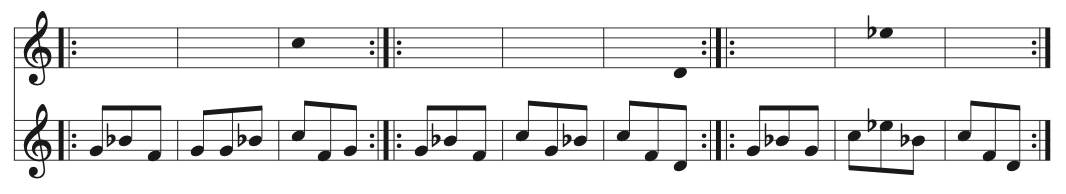
\includegraphics[width=0.7\textwidth]{images/obra5.png}
    \caption{Neste excerto da secção 5, observa-se a sobreposição da repetição no domínio do tempo, através das figuras de colcheia, com a quietude do campo harmónico, que se mostra diferente sempre que é dado um novo aperto de mão.}
    \label{fig:obra5}
\end{figure}

O desenlaçe posterior significa uma quebra por meio de inconsistências das repetições sentidas no domínio do tempo, que a conduz à eventual rutura do desenvolvimento criado, que devolve o músico ao estado energético inicial de apenas uma pulsação que, com o aprofundamento da quietude final, se vai aproximando do silêncio através da assímptota da dilatação temporal e do espaço, com a ajuda de movimentos realizados pelo intérprete.

Esta última secção não tem participação do público e as preparações emitem apenas vários objetos de complexidade tímbrica, representativos dos apertos de mão criados ao longo do exercício. Assim, apenas quando uma nova nota é introduzida no campo harmónico presente é que é intrepertada pelo \textsl{patch} de preparações, que constitui apenas um Direct e um Synchronic ligado a um Blendronic (Figura \ref{fig:bit5}).

\begin{figure}[h]
    \centering
    \captionsetup{width=0.8\textwidth}
    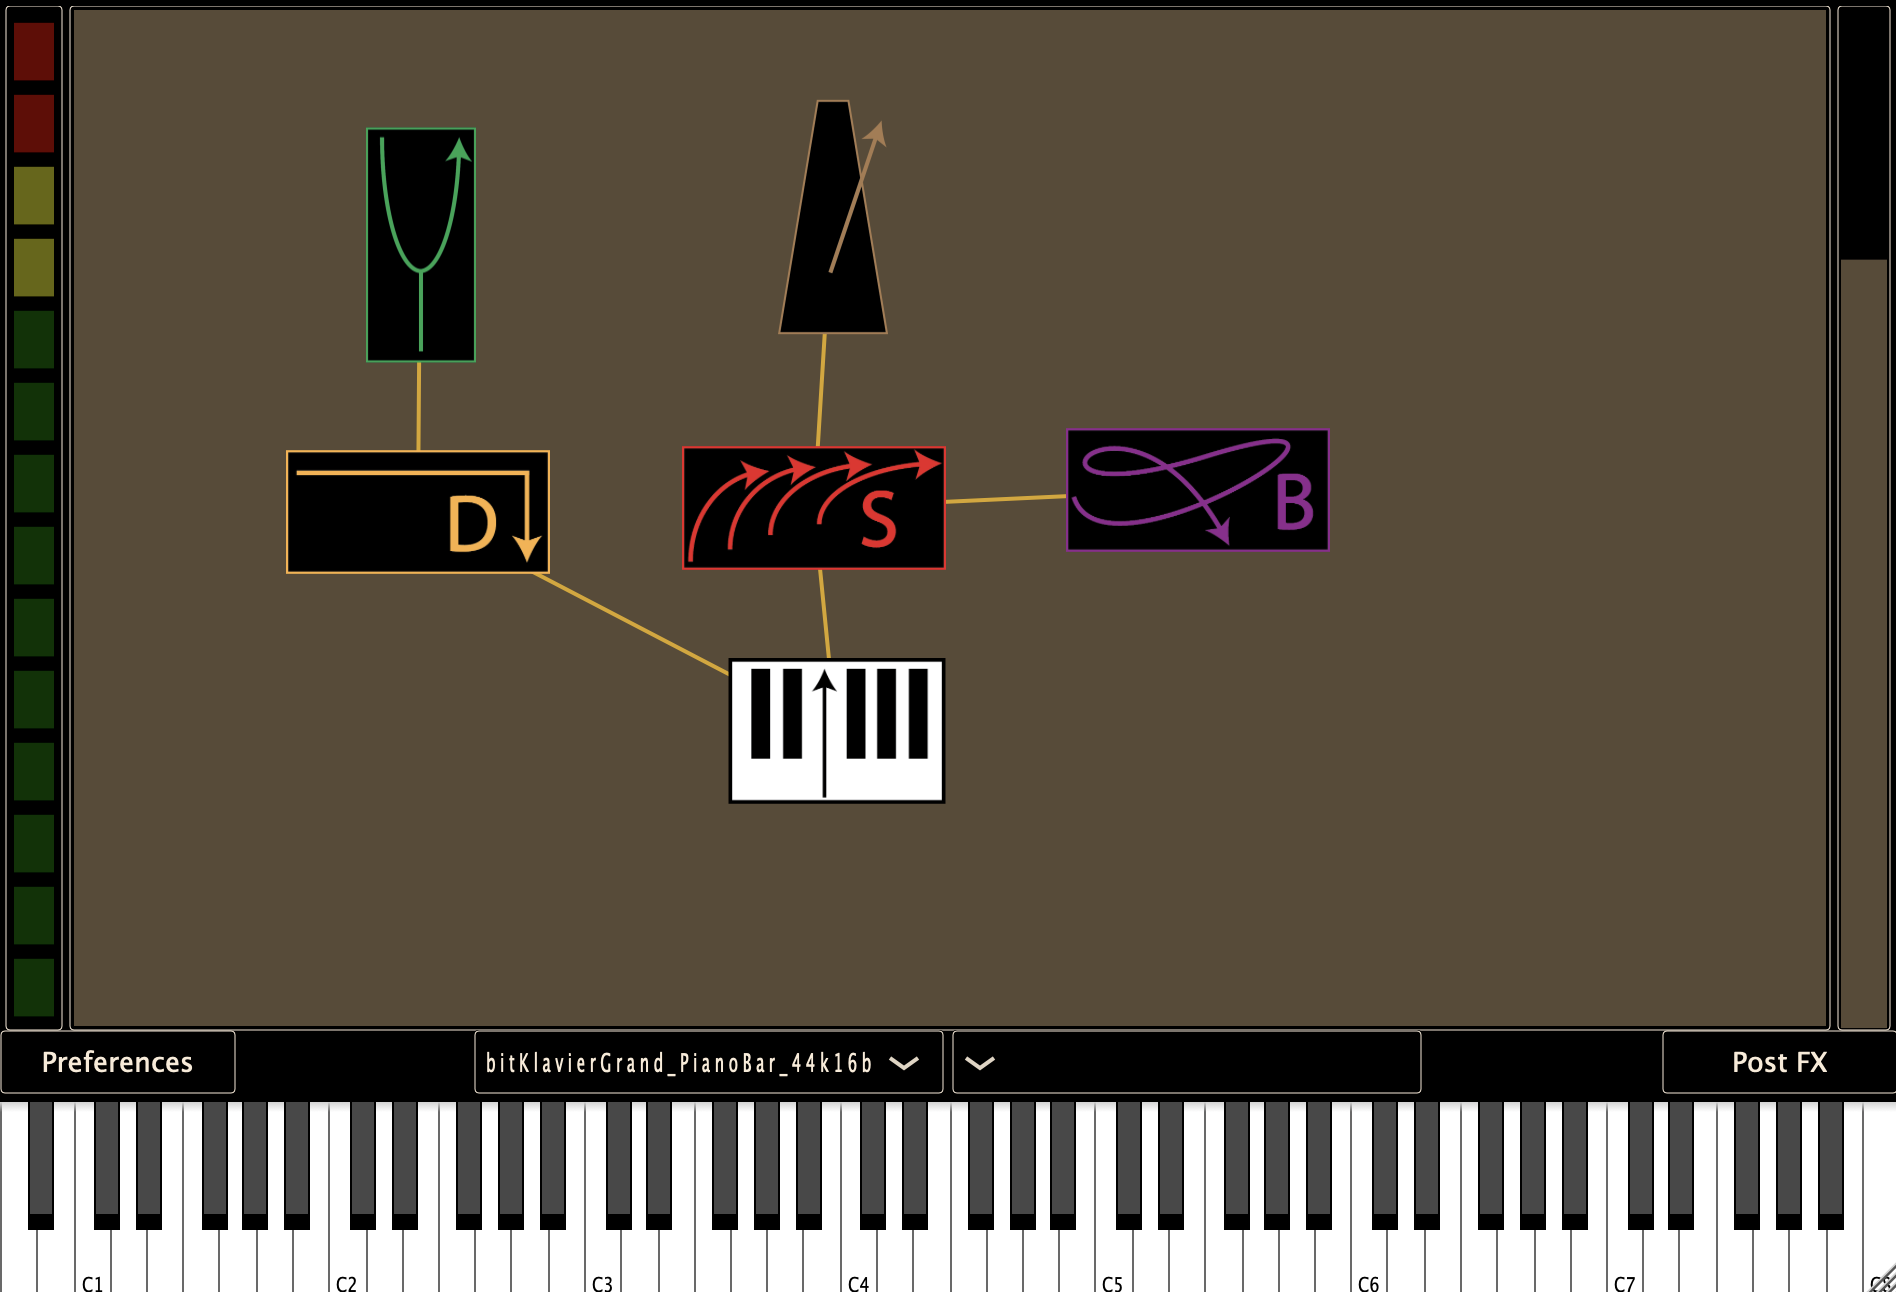
\includegraphics[width=0.7\textwidth]{images/bit5.png}
    \caption{\textsl{Patch} da secção 5. As notas disponíveis no Keymap correspondem apenas às notas referidas na partitura, de modo a atribuir uma textura musical representativa do aperto de mão referido no exercício, por meio das preparações Direct, Synchronic e Blendronic.}
    \label{fig:bit5}
\end{figure}

\Subsubsection{VI - O Fim?}
A obra termina com o músico a levantar-se repentinamente durante as incessáveis pulsações que encerram a última secção e a dirigir-se ao envelope, procurando atiçar uma última vez a curiosidade do público. Abrindo o envelope, estará escrito um último exercício performático de curta duração, de que o músico (ou qualquer outra pessoa) não poderá ter conhecimento. O exercício é um de entre os seguintes:
\begin{enumerate}
    \item Poisa o envelope. Volta para o piano. Finge que vais começar a tocar de novo. Volta a pegar no envelope. Volta para o envelope. Não toques, foge!
    \item Assusta-te sem fazer barulho. Coloca o papel dentro do envelope. Rasga o envelope 6 vezes no chão. Senta-te em cima dos pedaços e aprofunda a quietude o mais longo que conseguires.
    \item Olha para alguém na fila da frente do público. Analisa essa pessoa por uns segundos. Dá-lhe o envelope. Rasga o papel 2 vezes. Pede o envelope de volta e coloca os pedaços lá dentro. Leva o envelope contigo para fora do palco.
    \item Olha fixamente para alguém do público. Fecha os olhos e abre de novo. Se a pessoa se estiver a rir, assusta-te. Se não estiver, expressa-te furioso. Em ambos os casos, foge!
    \item Olha para o papel. Finge que não sabes ler. Abandona o palco com o papel e deixa o envelope.
    \item Olha para o papel. Não tires os olhos do papel. Aprofunda a quietude o mais longo que conseguires.
    \item Olha para o papel, olha para alguém do público. Repete. Não tem de ser para a mesma pessoa. Repete. Repete. Repete o maior número de vezes que conseguires.
    \item Poisa o envelope, volta a repetir o exercício do início, mas desta vez não estás sozinho na sala.
    \item \textsl{(folha em branco)}
\end{enumerate}

A execução deste exerício marca o final da obra, cuja inclareza vai de encontro com o conceito geral da obra, pois, não só o público não tem qualquer conhecimento do conteúdo do envelope, como também não conhecimento de que este momento representa o final da obra. No entanto, o prolongamento do silêncio terá o mesmo destino que o objeto do exerício da secção 0: mesmo um silêncio de grande complexidade, com o tempo, perde a energia que o concretiza. Assim que isso aconteça na perspectiva do músico, este pode dar por terminada a performance.

\end{document}